% Name: ROC curve
% Description: Receiver operating characteristic curves of two classifiers against the diagonal of chance, with the area under each curve in the legend.
% Tags: ROC curve, classification, AUC, machine learning

\usepackage{pgfplots}
\pgfplotsset{compat=1.18}

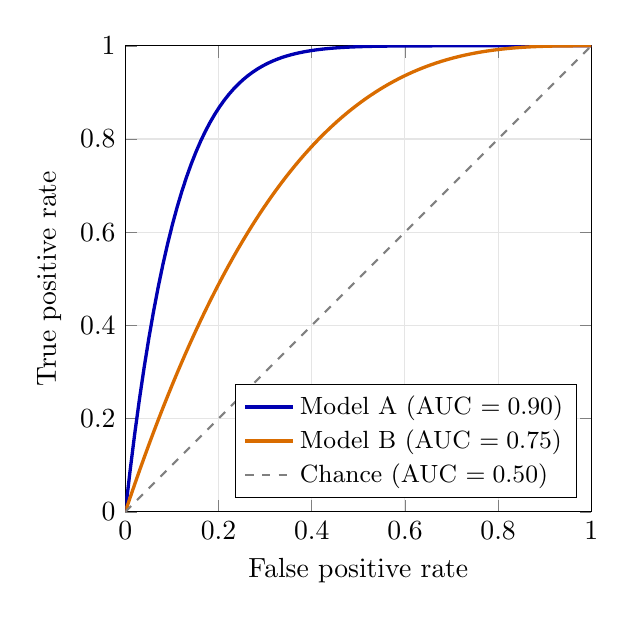
\begin{tikzpicture}
  \begin{axis}[
    width=7.5cm, height=7.5cm, xmin=0, xmax=1, ymin=0, ymax=1,
    xlabel={False positive rate}, ylabel={True positive rate},
    xtick={0,0.2,...,1}, ytick={0,0.2,...,1}, domain=0:1, samples=100,
    legend pos=south east, legend cell align=left, legend style={font=\small},
    grid=major, grid style={gray!20},
  ]
    % The curve y = 1 - (1 - x)^k has area k/(k + 1) under it.
    \addplot[very thick, blue!70!black] {1 - (1 - x)^9};
    \addplot[very thick, orange!85!black] {1 - (1 - x)^3};
    \addplot[thick, dashed, gray] {x};
    \legend{Model A (AUC $= 0.90$), Model B (AUC $= 0.75$), Chance (AUC $= 0.50$)}
  \end{axis}
\end{tikzpicture}
